\section{Example results}
%Olli

Figure \ref{fig:sampleResults} shows some screenshots from the Chrome extension. In it, the user is browsing Spiegel and has selected some text (see A on the left side). After clicking ``Search for entities'', the popup on the right appears with additional information about entities in the marked text. In this case, two entities \texttt{Merkel} (see A and B) and Germany (see C) have been found. For \texttt{Merkel}, several similar values for \textit{abstract} have been found (see B at the bottom). These can be expanded by clicking. The last picture (D) visualizes the connections between the two entities. Big circles (orange and purple) represent subjects and objects of triples while the smaller circles (light blue) represent the names of relations. 



\begin{figure}[H]
	\centering
	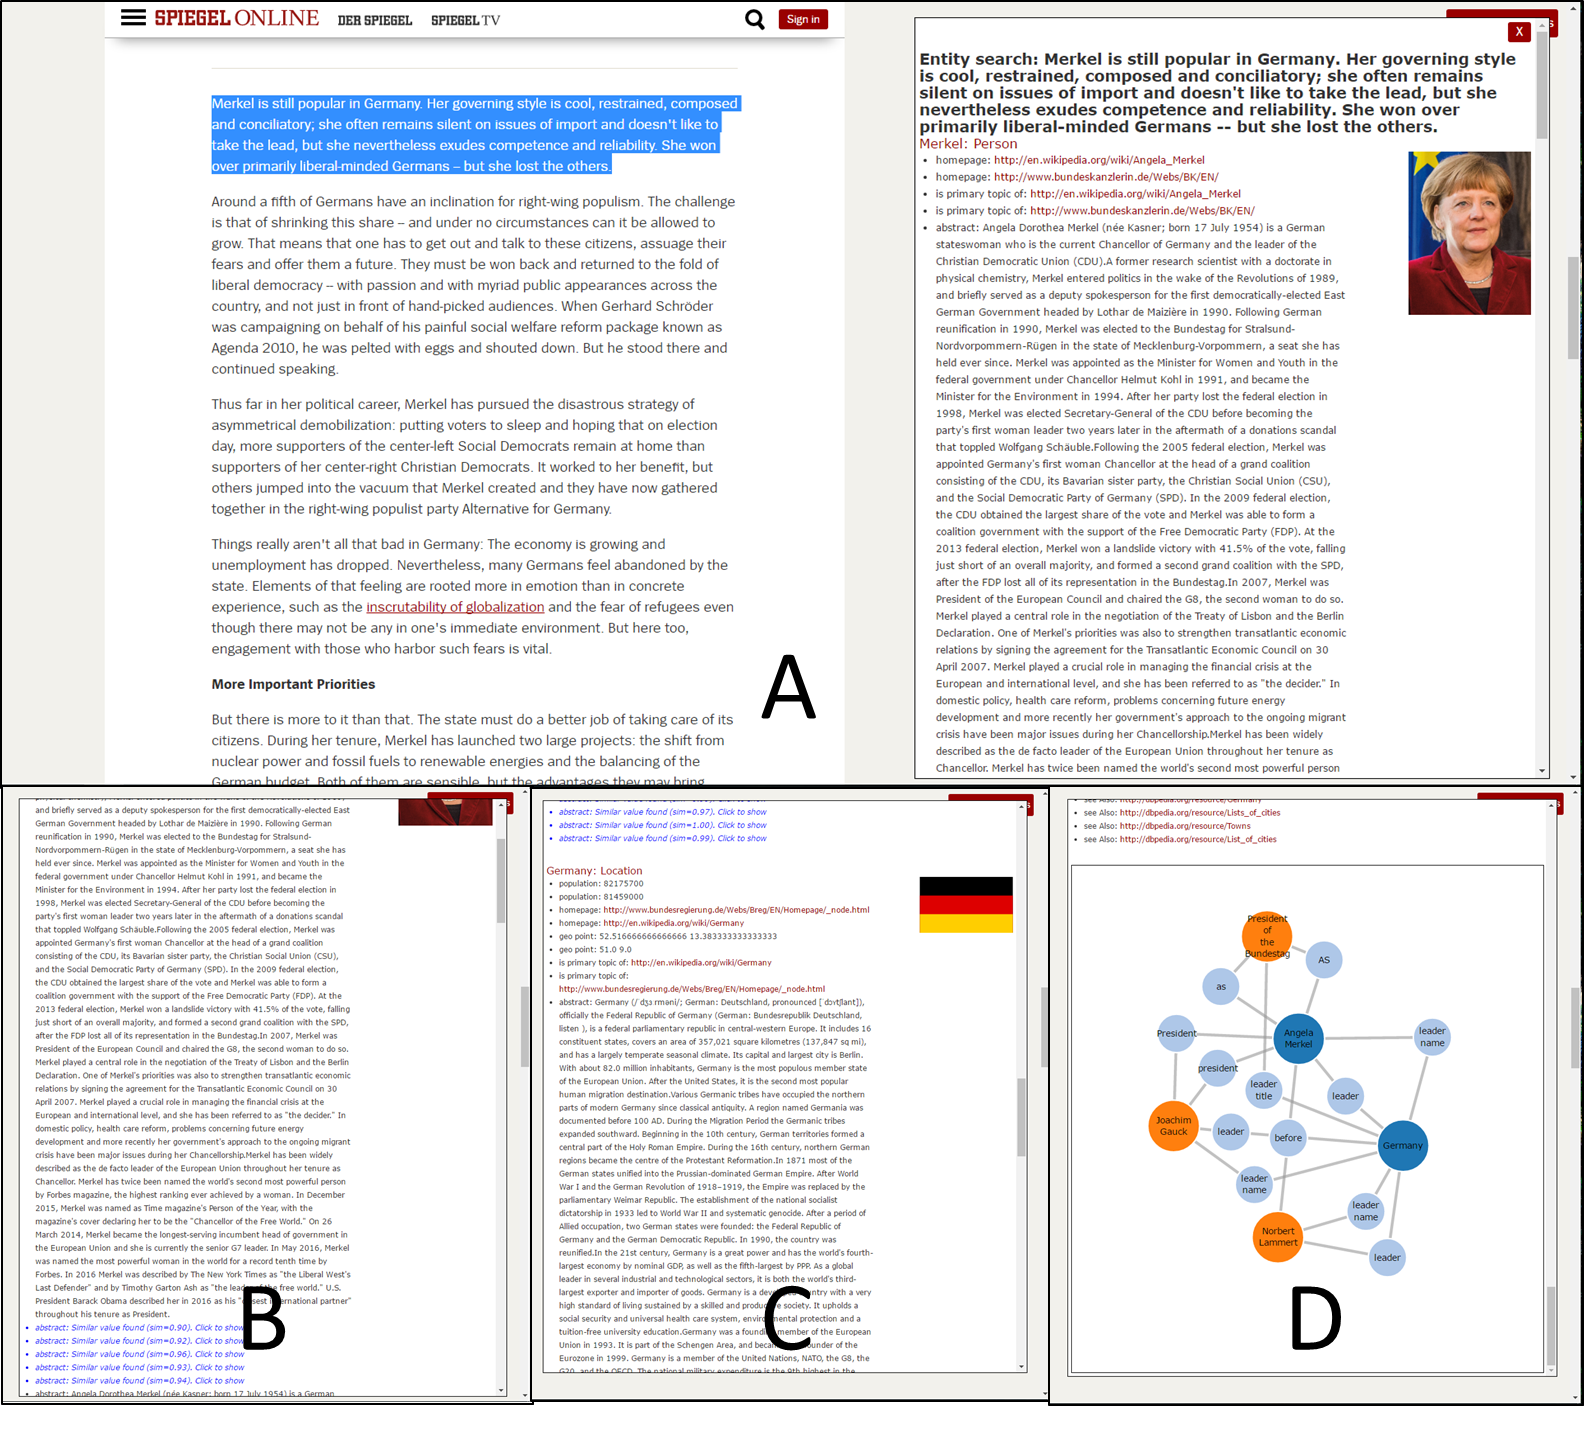
\includegraphics[width=1\textwidth]{img/sampleResults/sampleResult}
	\caption{Sample result}
	\label{fig:sampleResults}
\end{figure}






